\usepackage{tcolorbox}
\tcbuselibrary{theorems}
\tcbuselibrary{skins}
\tcbuselibrary{breakable}
%\newtcbtheorem[number within=section]{esempiot}{Esempio}%
%{fonttitle=\bfseries}{th}
%\newtcbtheorem [number within=section]{esempiot}{Esempio}{esestyle}{}
\tcbset{
defstyle/.style={enhanced,
                breakable,
                fonttitle=\bfseries\upshape,
                separator sign={.},
                colback=red!5!white,
                colframe=red!75!black,
                shadow={1mm}{-1mm}{0mm}{black!25!white}},                
esestyle/.style={enhanced,
                  breakable,
                   colback=white,
                    colbacktitle=gray!30,
                    coltitle=black,
                  fonttitle=\bfseries\upshape,
                  separator sign={.},
                  %colback=aliceblue,
                 % colframe=RoyalBlue,
                  shadow={0mm}{0mm}{0mm}{black!25!white}},
esestyleatt/.style={enhanced,
                  breakable,
                   colback=white,
                    colbacktitle=gray!20,
                    coltitle=black,
                  fonttitle=\bfseries\upshape,
                  separator sign={.},
                  colframe=white,
                  %colback=aliceblue,
                 % colframe=RoyalBlue,
                 borderline={0.5pt}{-5pt}{green},
                 % shadow={0mm}{0mm}{0mm}{black!25!white},
                 leftrule=12mm,
                  overlay={\node[anchor=north west,outer sep=2pt] at (frame.north west) {\includegraphics[width=8mm]{../Mod_base/0022}}; }
                  },
ossstyle/.style={enhanced,
                  breakable,
                  fonttitle=\bfseries\upshape,
                  separator sign={.},
                  colback=green!10,
                  colframe=green!50!black,
                  enlarge top by=5.5mm,
                  overlay={\foreach \x in {2cm,3.5cm} {
                     \begin{scope} [shift={([xshift=\x]frame.north west)}]
                     \path [draw=green!50!black,fill=green!10,line width=1mm] (0,0) arc (0:180:5mm);
                     \path [fill=black] (-0.2,0) arc (0:180:1mm);
                     \end{scope}}}],
                  shadow={1mm}{-1mm}{0mm}{black!25!white}},
procstyle/.style={enhanced,
                  breakable,
                  fonttitle=\bfseries\upshape,
                  separator sign={.},
                  colback=red!15!yellow!5!white,
                  colframe=orange!75!black,
                  shadow={1mm}{-1mm}{0mm}{black!25!white}},
princstyle/.style={enhanced,
                  breakable,
                  fonttitle=\bfseries\upshape,
                  separator sign={.},
                  colback=white!95!black,
                  colframe=black!75!white,
                  shadow={1mm}{-1mm}{0mm}{black!25!white}},
}
\newtcolorbox{lattention}{breakable,enhanced,arc=0mm,colback=gray!5,colframe=gray,leftrule=12mm,%
overlay={\node[anchor=north west,outer sep=2pt] at (frame.north west) {\includegraphics[width=8mm]{0022}}; }}

\newtcbtheorem [number within=chapter]{esempiot}{Esercizio}{esestyle}{}
\newtcbtheorem [number within=chapter] {definizionet}{Definizione}{defstyle}{}
\newtcbtheorem [number within=chapter] {procedurat}{Procedura}{procstyle}{}
\newtcbtheorem [number within=chapter] {osservazionet}{Osservazione}{ossstyle}{}
\newtcbtheorem [number within=chapter] {principiot}{Principio}{princstyle}{}